\documentclass[11pt]{article}
\usepackage[T1]{fontenc}
\usepackage{amsmath,amssymb,amsthm}
\usepackage{geometry}
\usepackage{graphicx}
\usepackage[hidelinks]{hyperref}
\geometry{margin=1in}

\newtheorem*{theorem}{Theorem}
\newtheorem*{remark}{Remark}

\newcommand{\BL}{\mathcal{BL}}
\newcommand{\Lone}{L_1}

\title{Removing the Sigma-Finite Hypothesis in an \(L_1\)-Amalgamation Lemma}
\author{Run \texttt{fa\_banach\_001}, agent \texttt{agent\_lane\_12}}
\date{2026-06-21}

\begin{document}
\sloppy
\maketitle

\section*{Source and Status}

This packet answers a specific question in Antonio Aviles and Pedro Tradacete,
\emph{Amalgamation and injectivity in Banach lattices}, arXiv:2007.15261.  The
status is
\[
  \texttt{full\_solution\_likely\_valid}
\]
for the sigma-finiteness-removal question after Lemma 4.2.

\section*{Source Question}

Lemma 4.2 of the source paper proves the following \(L_1\)-amalgamation result
under the assumption that the common measure \(\nu_0\) is \(\sigma\)-finite:
if
\[
  u_i:\Lone(\nu_0)\longrightarrow \Lone(\nu_i),\qquad i=1,2,
\]
are lattice isometric embeddings, then there are a positive measure \(\nu_3\)
and lattice isometric embeddings
\[
  v_i:\Lone(\nu_i)\longrightarrow \Lone(\nu_3),\qquad i=1,2,
\]
such that \(v_1u_1=v_2u_2\).

\begin{center}
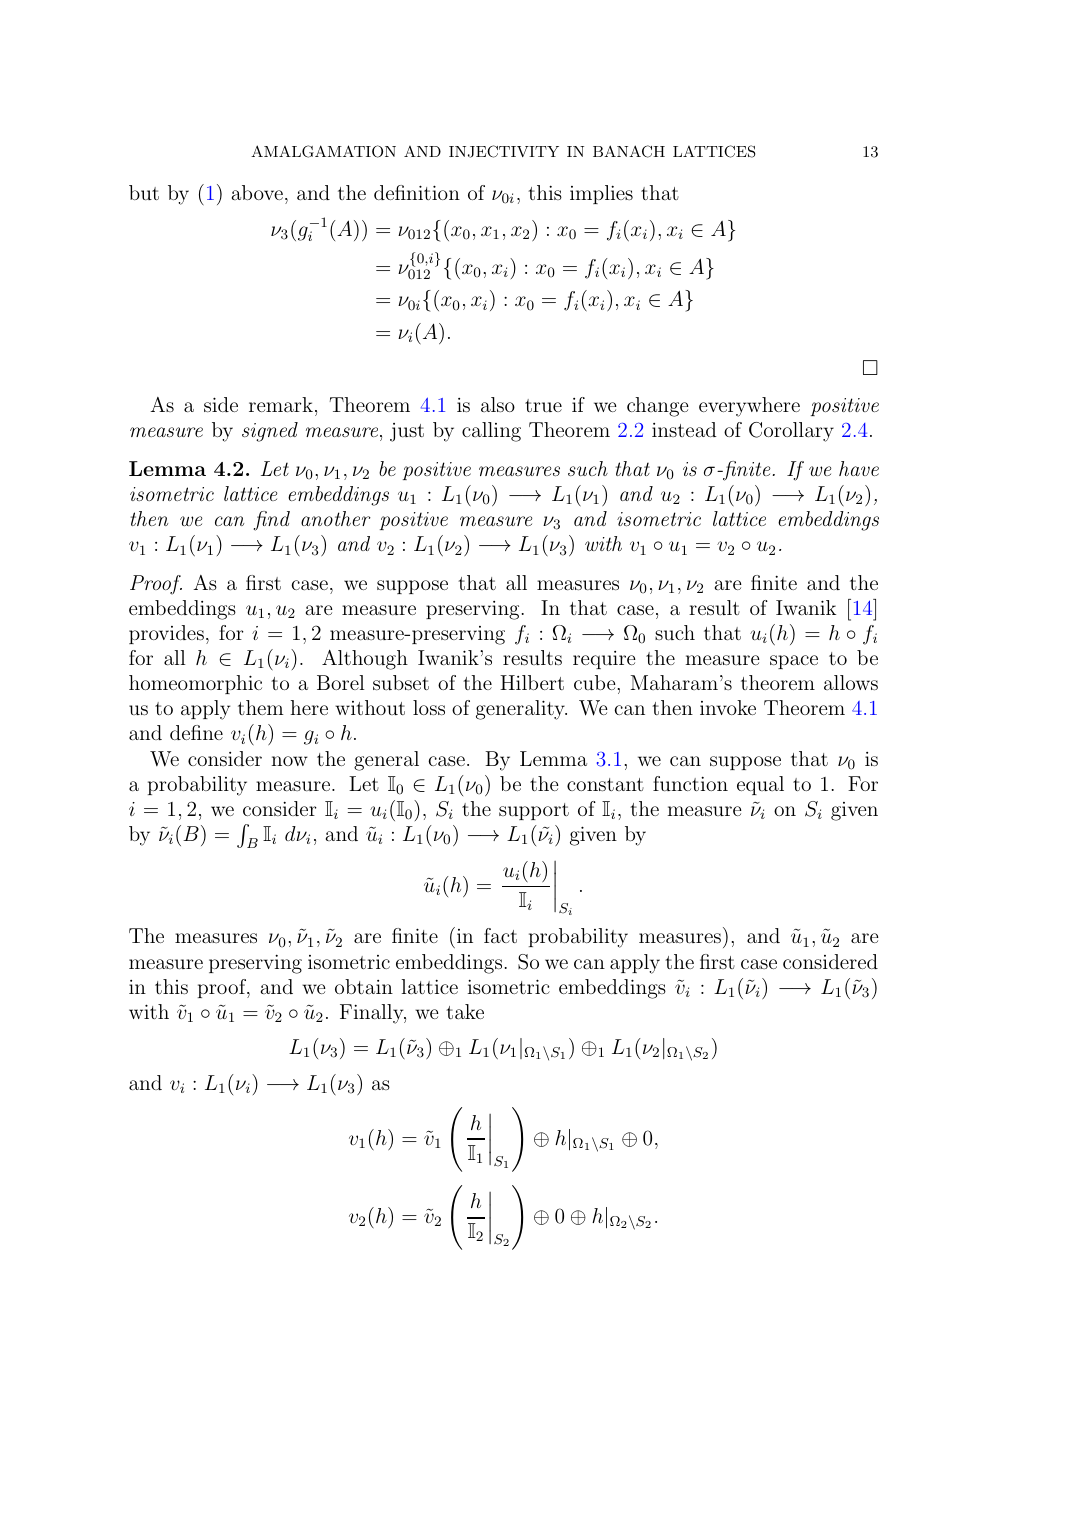
\includegraphics[width=.92\linewidth]{figures/l1_amalgamation_lemma_page13.png}
\end{center}

Immediately after the lemma, the authors ask whether the technical
\(\sigma\)-finiteness assumption on \(\nu_0\) can be removed.

\begin{center}
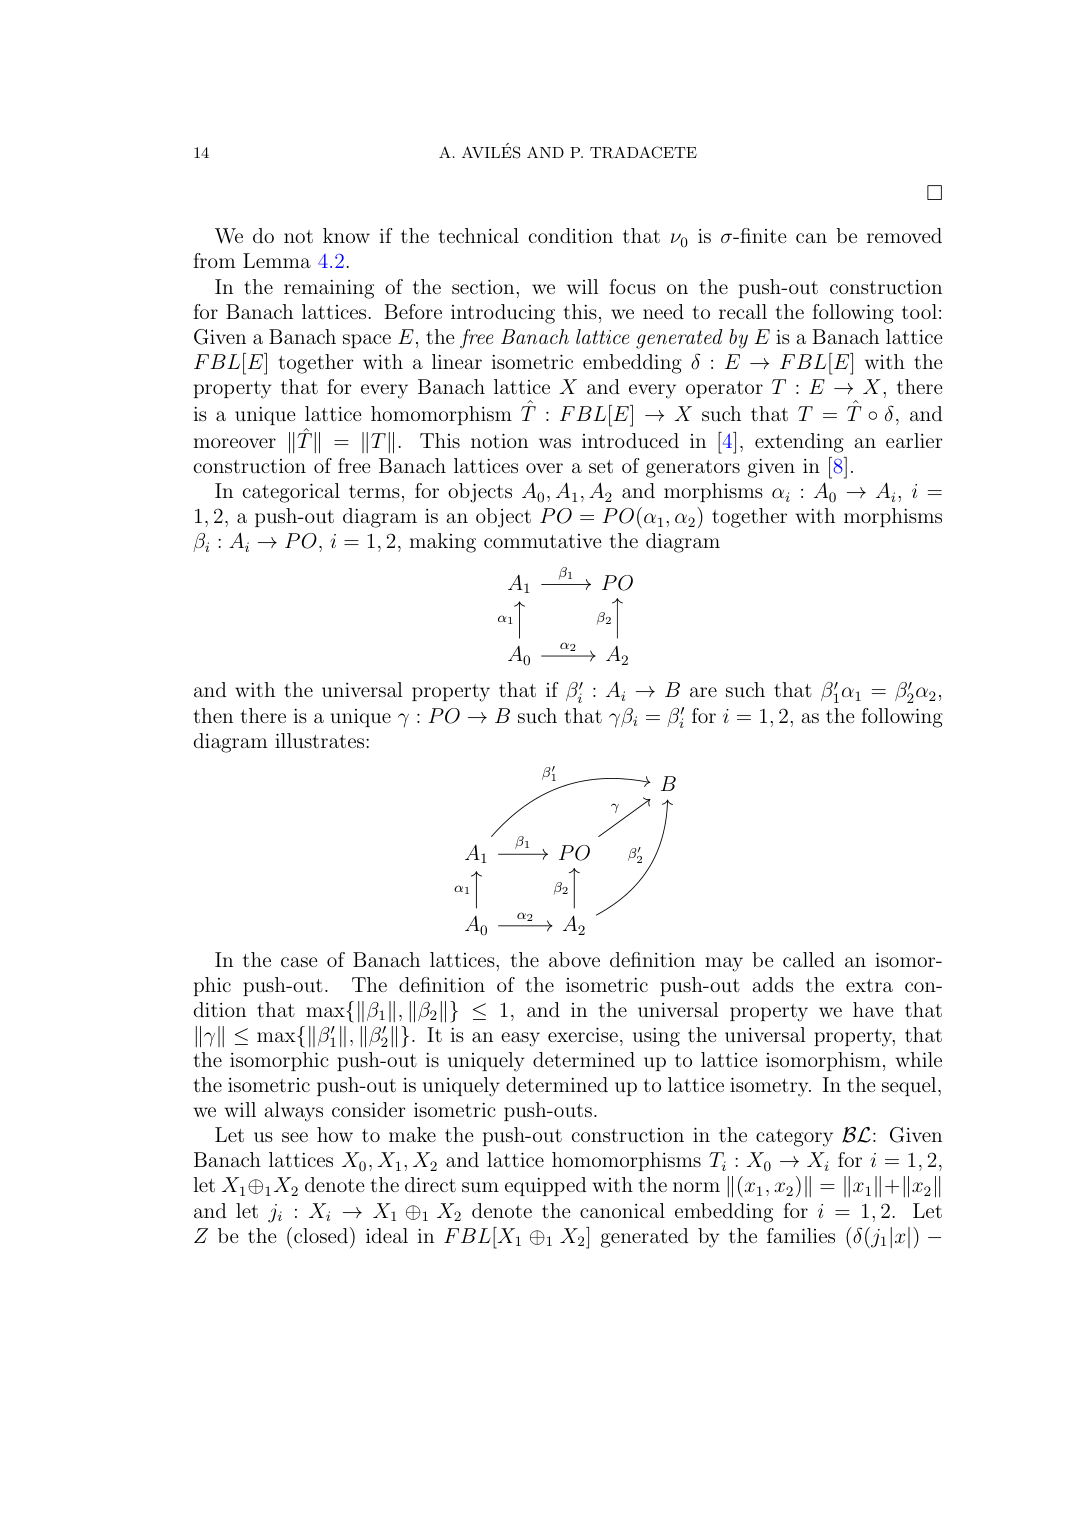
\includegraphics[width=.92\linewidth]{figures/sigma_finite_question_page14.png}
\end{center}

\section*{Idea of the Proof}

The only obstruction to directly applying Lemma 4.2 is that the common
\(L_1(\nu_0)\) may have no weak unit.  Maharam's theorem decomposes any
\(L_1\) space as an \(\ell_1\)-sum of standard pieces, each of which is
\(\sigma\)-finite: one-dimensional atomic pieces and finite-measure product
pieces \(L_1([0,1]^\kappa)\).  We apply the source lemma on each component.

Because lattice homomorphisms preserve disjointness, the images of distinct
components generate pairwise disjoint bands in each codomain.  After
amalgamating component by component, we take the \(\ell_1\)-sum of the
component amalgams and add the two residual codomain bands.  This sum is again
an \(L_1\) space, and it gives the desired global amalgamation.

\begin{center}
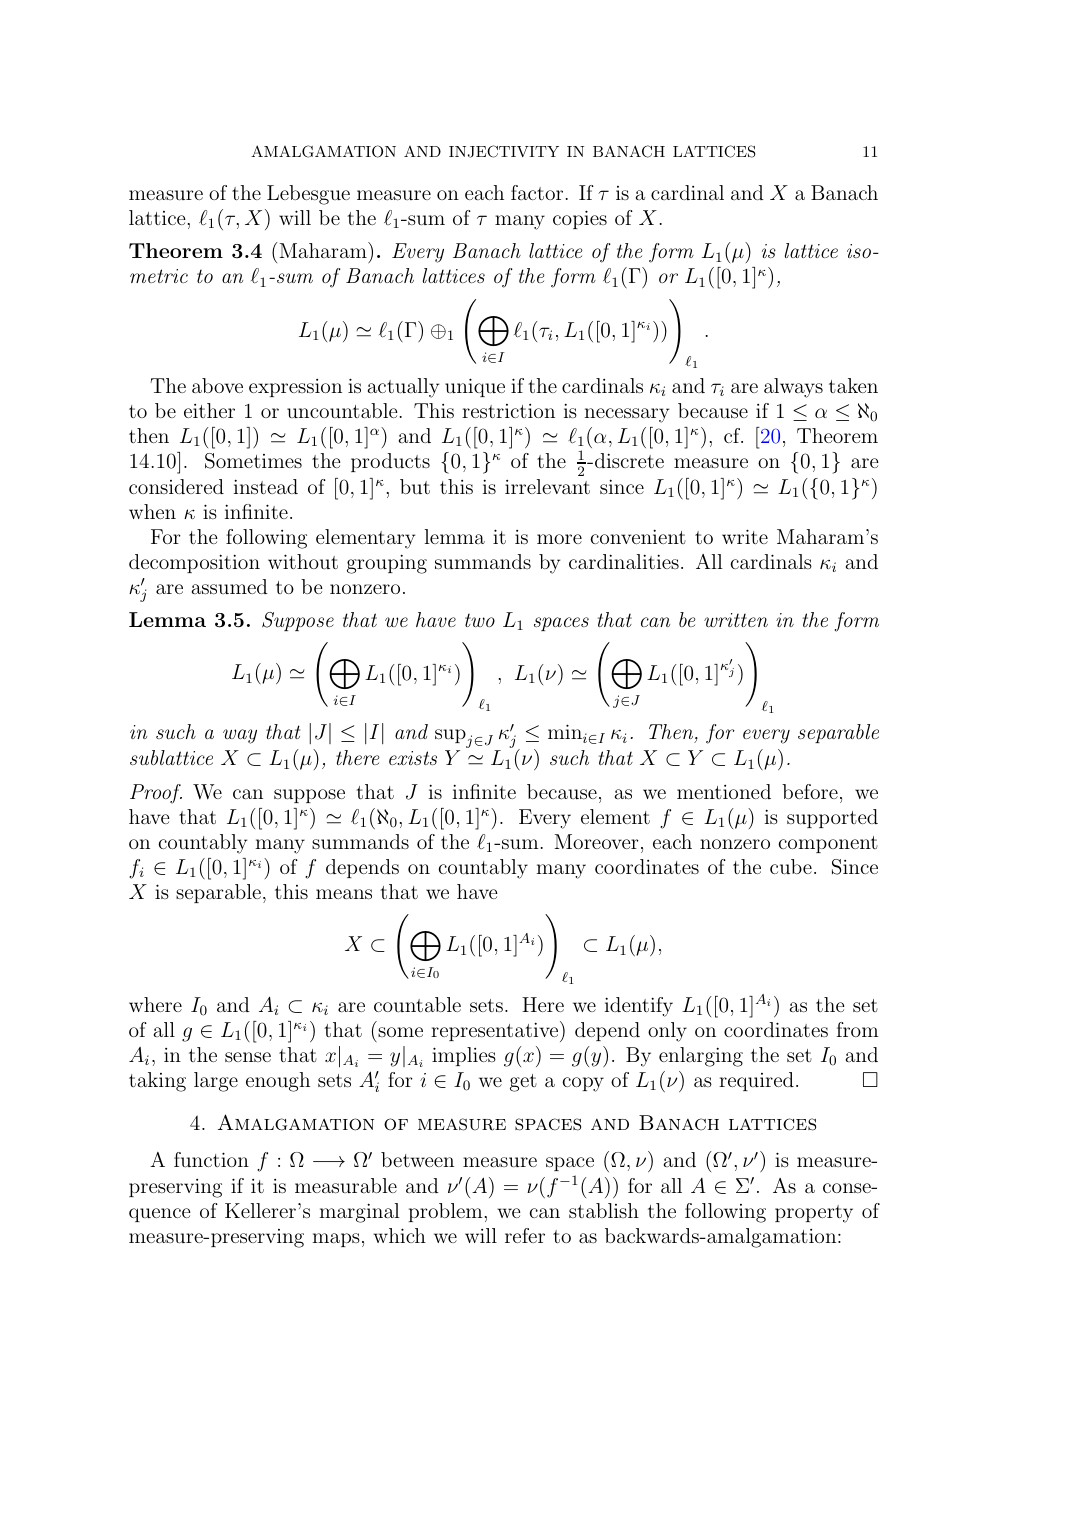
\includegraphics[width=.92\linewidth]{figures/maharam_decomposition_page11.png}
\end{center}

\section*{Main Result}

\begin{theorem}
Let \(\nu_0,\nu_1,\nu_2\) be arbitrary positive measures.  If
\[
  u_i:\Lone(\nu_0)\longrightarrow \Lone(\nu_i),\qquad i=1,2,
\]
are lattice isometric embeddings, then there exist a positive measure \(\nu_3\)
and lattice isometric embeddings
\[
  v_i:\Lone(\nu_i)\longrightarrow \Lone(\nu_3),\qquad i=1,2,
\]
such that
\[
  v_1u_1=v_2u_2.
\]
Thus the \(\sigma\)-finiteness hypothesis on \(\nu_0\) in Lemma 4.2 of the
source paper is unnecessary.
\end{theorem}

\begin{proof}
We use standard facts about abstract \(L_1\) spaces: bands generated by
pairwise disjoint positive elements decompose as \(\ell_1\)-sums, principal
bands generated by weak units are \(L_1\) spaces over \(\sigma\)-finite
measures, and \(\ell_1\)-sums of \(L_1\) spaces are again \(L_1\) spaces over
the disjoint union measure.

By Maharam's theorem, in the form quoted as Theorem 3.4 in the source paper,
we may write
\[
  \Lone(\nu_0)=\left(\bigoplus_{\alpha\in A} E_\alpha\right)_{\ell_1},
\]
where each \(E_\alpha\) is lattice isometric either to a one-dimensional
atomic \(L_1\) space or to \(L_1([0,1]^{\kappa_\alpha})\) with its product
probability measure.  In particular, every \(E_\alpha\) is an \(L_1\) space
over a \(\sigma\)-finite measure and has a positive weak unit \(e_\alpha\).

Fix \(i=1,2\).  Since \(u_i\) is a lattice homomorphism, the positive elements
\[
  b_{i,\alpha}=u_i(e_\alpha),\qquad \alpha\in A,
\]
are pairwise disjoint in \(\Lone(\nu_i)\).  Let \(F_{i,\alpha}\) be the
principal band generated by \(b_{i,\alpha}\).  Then the bands
\((F_{i,\alpha})_{\alpha\in A}\) are pairwise disjoint.  Also
\[
  u_i(E_\alpha)\subset F_{i,\alpha}.
\]
Indeed, if \(x\in E_\alpha\), then \(|x|\) belongs to the principal band
generated by \(e_\alpha\); equivalently,
\[
  |x|=\lim_{n\to\infty}(|x|\wedge n e_\alpha)
\]
in the \(L_1\)-norm.  Applying the lattice homomorphism \(u_i\) gives
\[
  |u_i x|
  =u_i|x|
  =\lim_{n\to\infty}u_i(|x|\wedge n e_\alpha),
\]
and each term is dominated by \(n b_{i,\alpha}\).  Hence \(u_i x\) lies in the
principal band \(F_{i,\alpha}\).

Let \(F_{i,0}\) be the band complement of the band generated by all
\((F_{i,\alpha})_{\alpha\in A}\).  Then
\[
  \Lone(\nu_i)=
  \left(\bigoplus_{\alpha\in A}F_{i,\alpha}\right)_{\ell_1}
  \oplus_1 F_{i,0}.
\]
Each \(F_{i,\alpha}\) is itself an \(L_1\) space, and the restricted maps
\[
  u_{i,\alpha}:E_\alpha\longrightarrow F_{i,\alpha}
\]
are lattice isometric embeddings.

Now apply Lemma 4.2 of the source paper to the pair
\[
  u_{1,\alpha}:E_\alpha\to F_{1,\alpha},\qquad
  u_{2,\alpha}:E_\alpha\to F_{2,\alpha}.
\]
The common domain \(E_\alpha\) is \(\sigma\)-finite, so the lemma gives an
\(L_1\) space \(W_\alpha\) and lattice isometric embeddings
\[
  r_{i,\alpha}:F_{i,\alpha}\longrightarrow W_\alpha,\qquad i=1,2,
\]
such that
\[
  r_{1,\alpha}u_{1,\alpha}=r_{2,\alpha}u_{2,\alpha}.
\]

Define
\[
  W=
  \left(\bigoplus_{\alpha\in A}W_\alpha\right)_{\ell_1}
  \oplus_1 F_{1,0}\oplus_1 F_{2,0}.
\]
This is an abstract \(L_1\) space, hence lattice isometric to \(L_1(\nu_3)\)
for some positive measure \(\nu_3\).  Define \(v_1:\Lone(\nu_1)\to W\) by
\[
  v_1\left((y_\alpha)_{\alpha\in A}\oplus y_0\right)
  =
  (r_{1,\alpha}y_\alpha)_{\alpha\in A}\oplus y_0\oplus 0,
\]
and define \(v_2:\Lone(\nu_2)\to W\) by
\[
  v_2\left((z_\alpha)_{\alpha\in A}\oplus z_0\right)
  =
  (r_{2,\alpha}z_\alpha)_{\alpha\in A}\oplus 0\oplus z_0.
\]
Both maps are lattice isometric embeddings.

Finally, if \(x=(x_\alpha)_{\alpha\in A}\in \Lone(\nu_0)\), then
\[
  u_i x=(u_{i,\alpha}x_\alpha)_{\alpha\in A}\oplus 0.
\]
Therefore
\[
  v_1u_1x
  =(r_{1,\alpha}u_{1,\alpha}x_\alpha)_{\alpha\in A}\oplus0\oplus0
  =(r_{2,\alpha}u_{2,\alpha}x_\alpha)_{\alpha\in A}\oplus0\oplus0
  =v_2u_2x.
\]
This completes the amalgamation without assuming that \(\nu_0\) is
\(\sigma\)-finite.
\end{proof}

\section*{Scope and Limitations}

This solves only the local question after Lemma 4.2: the \(L_1\)-amalgamation
lemma remains true for arbitrary common \(L_1(\nu_0)\).  It does not resolve
the later question in the paper about whether every separably \(\BL\)-injective
Banach lattice is isomorphic to a \(1\)-separably \(\BL\)-injective one.

\section*{Novelty Check}

Before promotion, the run indexes were searched for arXiv:2007.15261, the
title, ``Banach lattice amalgamation'', ``injective Banach lattice'', and
related amalgamation keywords.  The only hits were broad amalgamation packets
for other papers and categories, not this \(L_1\)-amalgamation condition.
External web search for the exact phrases around the sigma-finiteness question
and for later references to the paper found the source paper but no later
answer to this specific question.

\section*{References}

\begin{itemize}
\item Antonio Aviles and Pedro Tradacete,
\emph{Amalgamation and injectivity in Banach lattices},
arXiv:2007.15261.
\item H. E. Lacey, \emph{The isometric theory of classical Banach spaces},
used through the Maharam classification quoted in the source paper.
\end{itemize}

\section*{Human Review Recommendation}

Review the standard band-decomposition step in the codomain \(L_1\) spaces:
the proof uses that pairwise disjoint principal bands in an abstract \(L_1\)
space form an \(\ell_1\)-summand together with their band complement.  With
that standard fact, the componentwise use of Lemma 4.2 gives a complete answer
to the source question.

\end{document}
